\documentclass[10pt]{article}

\usepackage[left=2cm, right=2cm, top=2cm, bottom=3cm]{geometry}

% Input encoding and typographical rules for English language
\usepackage[utf8]{inputenc}
\usepackage[english]{babel}
\usepackage[english]{isodate}

% More defined colors
\usepackage[dvipsnames]{xcolor}

% Required package
\usepackage{tikz}
\usetikzlibrary{arrows, arrows.meta, decorations.markings, shapes.geometric}
\usetikzlibrary{positioning}

\tikzstyle{dbusarrow} = [
    thick,
    decoration={
        markings,
        mark=at position 0 with {\arrowreversed[semithick]{open triangle 60}},
        mark=at position 1 with {\arrow[semithick]{open triangle 60}}
    },
    double distance=1.4pt,
    shorten >= 5.5pt,
    shorten <= 5.5pt,
    preaction = {decorate},
    postaction = {draw,line width=1.4pt, white,shorten >= 4.5pt, shorten <= 4.5pt}
]

\usepackage{enumitem}
\usepackage{multicol}

\makeatletter
\renewcommand{\maketitle}{
{\Huge\textbf{\@title}} \\
\noindent\rule{\textwidth}{1pt} \\
\medskip
}
\makeatother

% Section header size and spacing
\makeatletter
\renewcommand{\section}{%
  \@startsection{section}{1}{0pt}{-3.5ex plus -1ex minus -.2ex}{2.3ex plus .2ex}{\Large\bfseries\sffamily}%
}
\makeatother

% No numbering for section titles
\setcounter{secnumdepth}{0}

% ============================================================================ %

% These define global texts that are used in headers and titles.
\title{mea-craft}
\author{Felipe Paiva Alencar}
\date{June 2023}
% \revision{Revision 1}

\begin{document}
\maketitle

\begin{multicols}{2}
\section{Features}
\begin{itemize}

\item \textbf{RISC-V Core:}
\begin{itemize}
\item DIY implementation of the RV32I instruction set architecture (ISA),
providing a flexible and customizable processing core.
\item Uses the AXI4-Lite memory interface enabling a seamless interface with
different memory devices.
\item Has support for interrupts allowing the implementation of event-driven
functionalities.
\end{itemize}

\item \textbf{Graphics:}
\begin{itemize}
\item The sprite architecture presented in class, has been enhanced to enable
dynamic changes to sprite contents, multiple texture scales, and memory sharing
between sprites.
\item Fully parametric, has support 80 sprites arranged in 5 clusters in the
default configuration.
\end{itemize}

\item \textbf{Memory:} 
\begin{itemize}
\item 4 kilobytes of ROM: Storing a small bootloader that also performs a quick
test of the ISA implementation.
\item 64 kilobytes of RAM: More than sufficient memory capacity to
handle game, texture, and world data.
\item 20.48 kilopixels of texture memory: arranged in 5 clusters of sprites.
\end{itemize}

\item \textbf{Peripherals:}
\begin{itemize}
\item General Purpose Input/Output (GPIO) that allows the interface of the
software with the buttons and switches. 
\item Universal asynchronous receiver-transmitter (UART) that provides a
communication channel.
\end{itemize}

\item \textbf{Build Tools:}
\begin{itemize}
\item The build and flashing process is efficiently automated by a well designed
Makefile, simplifying the compilation, texture packaging, world generation, and
linking tasks.
\item Support for bulding and flashing via a single command, saving valuable
development time and effort.
\end{itemize}

\end{itemize}
\end{multicols}

\pagebreak

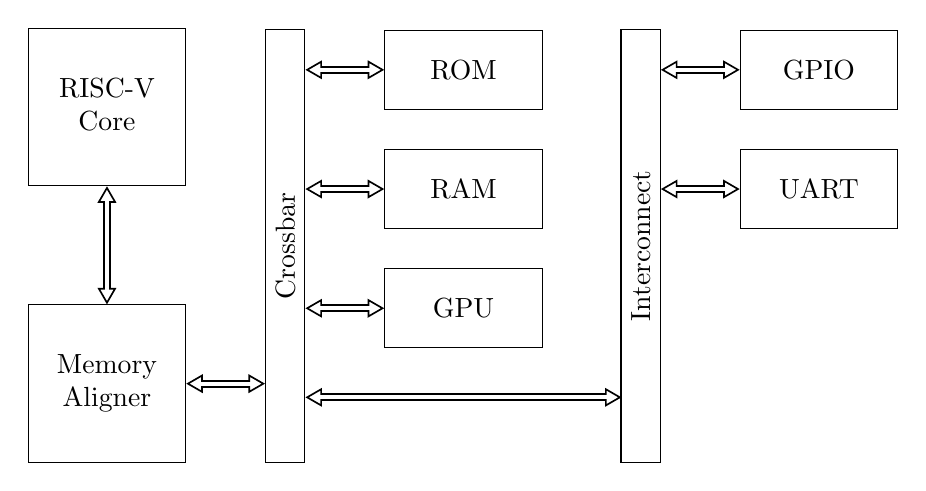
\begin{tikzpicture}

\node [draw,
    minimum width=2cm,
    minimum height=2cm,
]  (core) {\begin{tabular}{c} RISC-V \\ Core \end{tabular}};

\node [draw,
    minimum width=2cm,
    minimum height=2cm,
    below=1.5cm of core
]  (aligner) {\begin{tabular}{c} Memory \\ Aligner \end{tabular}};

\node [draw,
    minimum width=0.5cm,
    minimum height=5.5cm,
    below right=-2cm and 1cm of core
]  (crossbar) {\rotatebox{90}{Crossbar}};

\node [draw,
    minimum width=2cm,
    minimum height=1cm,
    below right=-5.5cm and 1cm of crossbar
]  (rom) {ROM};

\node [draw,
    minimum width=2cm,
    minimum height=1cm,
    below=0.5cm of rom
]  (ram) {RAM};

\node [draw,
    minimum width=2cm,
    minimum height=1cm,
    below=0.5cm of ram
]  (gpu) {GPU};

\node [draw,
    minimum width=0.5cm,
    minimum height=5.5cm,
    right=4cm of crossbar
]  (interconnect) {\rotatebox{90}{Interconnect}};

\node [draw,
    minimum width=2cm,
    minimum height=1cm,
    below right=-5.5cm and 1cm of interconnect
]  (gpio) {GPIO};

\node [draw,
    minimum width=2cm,
    minimum height=1cm,
    below=0.5cm of gpio
]  (uart) {UART};

\draw[dbusarrow] (core.south) -- (aligner.north);

\node[right=1cm of aligner] (ref0) {};
\draw[dbusarrow] (aligner.east) -- (ref0);

\node[left=1cm of rom] (ref1) {};
\draw[dbusarrow] (rom.west) -- (ref1);

\node[left=1cm of ram] (ref2) {};
\draw[dbusarrow] (ram.west) -- (ref2);

\node[left=1cm of gpu] (ref3) {};
\draw[dbusarrow] (gpu.west) -- (ref3);

\node[below left=0.5cm and 1cm of gpu] (ref4) {};
\node[below right=0.5cm and 1cm of gpu] (ref5) {};
\draw[dbusarrow] (ref4) -- (ref5);

\node[left=1cm of gpio] (ref6) {};
\draw[dbusarrow] (gpio.west) -- (ref6);

\node[left=1cm of uart] (ref7) {};
\draw[dbusarrow] (uart.west) -- (ref7);
    
\end{tikzpicture}

\pagebreak

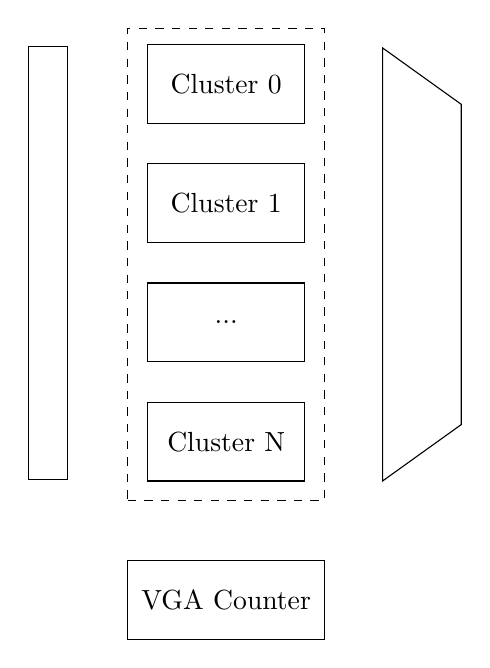
\begin{tikzpicture}

\node [draw,
    minimum width=2cm,
    minimum height=1cm,
] (cluster_0) {Cluster 0};

\node [draw,
    minimum width=2cm,
    minimum height=1cm,
    below=0.5cm of cluster_0
] (cluster_1) {Cluster 1};

\node [draw,
    minimum width=2cm,
    minimum height=1cm,
    below=0.5cm of cluster_1
] (cluster_dot) {...};

\node [draw,
    minimum width=2cm,
    minimum height=1cm,
    below=0.5cm of cluster_dot
] (cluster_n) {Cluster N};

\node [draw,
    dashed,
    minimum width=2.5cm,
    minimum height=6cm,
    rotate=180,
    below right=0.25cm and 0.25cm of cluster_n
] (clusters) {};

\node [draw,
    minimum width=2.5cm,
    minimum height=1cm,
    below=1cm of cluster_n
] (vga) {VGA Counter};

\node [draw,
    minimum width=0.5cm,
    minimum height=5.5cm,
    below left=-2.5cm and 1cm of cluster_1
] (interconnect) {};

\node[draw,
    shape=trapezium,
    trapezium left angle=80,
    trapezium right angle=80,
    rotate=-90,
    minimum width=5.5cm,
    minimum height=1cm,
    trapezium stretches=true,
    below right=-3.25cm and 5cm of interconnect
] (mux) {};

% \node [draw,
%     shape=trapezium,
%     rotate=-90,
%     minimum width=0.5cm,
%     minimum height=5.5cm,
%     below right=-2.5cm and 1cm of cluster_1
% ] (mux) {};

\end{tikzpicture}

\end{document}


